%\special{!userdict begin /bop-hook{gsave 200 30 translate
%       65 rotate /Times-Roman findfont 216 scalefont setfont
%       0 0 moveto 0.85 setgray (DRAFT) show grestore}def end}

\documentclass[11pt,a4paper]{article}

\usepackage{graphicx}
\usepackage{float}
\usepackage{afterpage}
\usepackage{epsfig,cite,multirow}
\usepackage{amssymb}
\usepackage{amsmath}
\usepackage{dsfont}
\usepackage{multirow}
\usepackage{epstopdf}
\usepackage{url,hyperref}
\usepackage{listings}

\lstset{frame=tb,
  language=bash,
  aboveskip=3mm,
  belowskip=3mm,
  showstringspaces=false,
  columns=flexible,
  basicstyle={\small\ttfamily},
  numbers=none,
  numberstyle=\tiny\color{gray},
  breaklines=true,
  breakatwhitespace=true,
  tabsize=3
}


%\textwidth=15.0cm \textheight=23.5cm
\textwidth=16.5cm \textheight=23.5cm 
\topmargin 0cm \oddsidemargin 0cm 
\setlength{\unitlength}{1mm}

\usepackage{url}
\usepackage{hyperref}

\bibliographystyle{JHEP}
%\bibliographystyle{plain}

%%%%%%%%%%%%%%%%%%%%%%%%%%%%%%%%%%%%%%%%%%%%%%%%%%%%%%%%%%%%%

\def\smallfrac#1#2{\hbox{$\frac{#1}{#2}$}}
\newcommand{\be}{\begin{equation}}
\newcommand{\ee}{\end{equation}}
\newcommand{\bea}{\begin{eqnarray}}
\newcommand{\eea}{\end{eqnarray}}
\newcommand{\bi}{\begin{itemize}}
\newcommand{\ei}{\end{itemize}}
\newcommand{\ben}{\begin{enumerate}}
\newcommand{\een}{\end{enumerate}}
\newcommand{\la}{\left\langle}
\newcommand{\ra}{\right\rangle}
\newcommand{\lc}{\left[}
\newcommand{\rc}{\right]}
\newcommand{\lp}{\left(}
\newcommand{\rp}{\right)}
\newcommand{\as}{\alpha_s}
\newcommand{\aq}{\alpha_s\left( Q^2 \right)}
\newcommand{\amz}{\alpha_s\left( M_Z^2 \right)}
\newcommand{\aqq}{\alpha_s \left( Q^2_0 \right)}
\newcommand{\aqz}{\alpha_s \left( Q^2_0 \right)}
\def\toinf#1{\mathrel{\mathop{\sim}\limits_{\scriptscriptstyle
{#1\rightarrow\infty }}}}
\def\tozero#1{\mathrel{\mathop{\sim}\limits_{\scriptscriptstyle
{#1\rightarrow0 }}}}
\def\toone#1{\mathrel{\mathop{\sim}\limits_{\scriptscriptstyle
{#1\rightarrow1 }}}}
\def\frac#1#2{{{#1}\over {#2}}}
\def\gsim{\mathrel{\rlap{\lower4pt\hbox{\hskip1pt$\sim$}}
    \raise1pt\hbox{$>$}}}         %greater than or approx. symbol
\def\lsim{\mathrel{\rlap{\lower4pt\hbox{\hskip1pt$\sim$}}
    \raise1pt\hbox{$<$}}}         %less than or approx. symbol
\newcommand{\mrexp}{\mathrm{exp}}
\newcommand{\dat}{\mathrm{dat}}
\newcommand{\one}{\mathrm{(1)}}
\newcommand{\two}{\mathrm{(2)}}
\newcommand{\art}{\mathrm{art}} 
\newcommand{\rep}{\mathrm{rep}}
\newcommand{\net}{\mathrm{net}}
\newcommand{\stopp}{\mathrm{stop}}
\newcommand{\sys}{\mathrm{sys}}
\newcommand{\stat}{\mathrm{stat}}
\newcommand{\diag}{\mathrm{diag}}
\newcommand{\pdf}{\mathrm{pdf}}
\newcommand{\tot}{\mathrm{tot}}
\newcommand{\minn}{\mathrm{min}}
\newcommand{\mut}{\mathrm{mut}}
\newcommand{\partt}{\mathrm{part}}
\newcommand{\dof}{\mathrm{dof}}
\newcommand{\NS}{\mathrm{NS}}
\newcommand{\cov}{\mathrm{cov}}
\newcommand{\gen}{\mathrm{gen}}
\newcommand{\cut}{\mathrm{cut}}
\newcommand{\parr}{\mathrm{par}}
\newcommand{\val}{\mathrm{val}}
\newcommand{\tr}{\mathrm{tr}}
\newcommand{\checkk}{\mathrm{check}}
\newcommand{\reff}{\mathrm{ref}}
\newcommand{\extra}{\mathrm{extra}}
\newcommand{\draft}[1]{}
\newcommand{\comment}[1]{{\bf \it  #1}}
\def\beq{\begin{equation}}  
\def\eeq{\end{equation}}  

% Added by MU for the fast evolution section
\def\bgamma{\boldsymbol{\gamma}}
\def\nn{\nonumber}
\def \so{\sigma_I^{DIS}(x_I,Q^2_I)}
\def \sh{\frac{d\sigma^{hh}}{dX}}
\def\sdy{\frac{d\sigma^{\mathrm{DY}}}{dQ_I^2dY_I}}
\def \npdf{N_{\mathrm{pdf}}}
\def \gtilda{\tilde\Gamma_J^{\mathrm{OBS}}}
\def \n0{N_j^{(0)}}
\def \a{\alpha}
\def \b{\beta}
\def \g{\gamma}
\def \c{\xi}
\def \z{\zeta}
% Added by JR
\def\lapprox{\lower .7ex\hbox{$\;\stackrel{\textstyle <}{\sim}\;$}}
\def\gapprox{\lower .7ex\hbox{$\;\stackrel{\textstyle >}{\sim}\;$}}
\def\half{\smallfrac{1}{2}}
\def\GeV{{\rm GeV}}
\def\TeV{{\rm TeV}}
\def\ap{{a'}}
\def\vp{{v'}}
\def\e{\epsilon}
\def\d{{\rm d}}
\def\calN{{\cal N}}
\def\shat{\hat{s}}
\def\barq{\bar{q}}
\def\qq{q \bar q}
\def\uu{u \bar u}
\def\dd{d \bar d}
\def\pp{p \bar p}
\def\xa{x_{1}}
\def\xb{x_{2}}
\def\xaa{x_{1}^{0}}
\def\xbb{x_{2}^{0}}
\def\smx{\stackrel{x\to 0}{\longrightarrow}}
\def\Li{{\rm Li}}

\newcommand{\tmop}[1]{\ensuremath{\operatorname{#1}}}
\newcommand{\tmtextit}[1]{{\itshape{#1}}}
\newcommand{\tmtextrm}[1]{{\rmfamily{#1}}}
\newcommand{\tmtexttt}[1]{{\ttfamily{#1}}}
\begin{document}

We thank the referee for the careful reading of our manuscript,
her/his positive appreciation of our work as well as for
her/his insightful comments, which have prompted us to study
in some detail some important aspects of our analysis.
%
In the following, we reply to each of the points raised by the
referee in turn.

\begin{itemize}

\item In the first comment, the referee states that:

  \begin{quote}
    \it
``It is certainly true that electroweak backgrounds such as $b\bar{b}Z(\to b\bar{b})$, $tth$ or $HZ$ are smaller than the QCD backgrounds, but they are also much bigger than the signal. A priori it is not clear to me that they can be neglected. Previous analyses, with which the authors compare their study, have included such backgrounds and found them relevant. I would ask the authors to show that after their reconstruction these backgrounds are significantly smaller than their signal process to be irrelevant for their significance. If the authors do not want to do a full study including those backgrounds it should suffice to use their final cuts and run over a set of events for each of these processes to show that they are well under control.'' 
    \end{quote}

  To address this point, we have generated additional background samples for
  the following single-Higgs
  processes:
  \begin{enumerate}
  \item $Z(\to b\bar{b})h(\to b\bar{b})$ (electroweak)
  \item $t\bar{t}h(\to b\bar{b})$
    \item $b\bar{b}h(\to b\bar{b})$ (QCD)
  \end{enumerate}
  For each of these additional background processes, we have generated 1M events using
  {\tt MadGraph5\_aMC@NLO} at leading order.
  %
  In Table~\ref{HK} of this note we list the
  LO and NLO cross-sections at the generation level for the single-Higgs background
  processes listed above.
  %
  The subsequent decays and the corresponding branching fractions are not included here, since
  these are taken care by the {\tt Pythia8} parton shower.
  %
  The values of these branching fractions applied to the single-Higgs
  background processes from Table~\ref{HK} of this note
  are listed in Table~\ref{HBF} below.
  %
  The values that we used are the most recent averages from the PDG.
  %
  In the case of the $t\bar{t}h$ process, we consider only the fully hadronic decays
  of the top quark, since leptonic and semi-leptonic decays can be discriminated
  by means of a lepton veto.
  
  %%%%%%%%%%%%%%%%%%%%%%%%%%%%%%%%%%%%%%%%%%%%
  %%%%%%%%%%%%%%%%%%%%%%%%%%%%%%%%%%%%%%%%%%%%
  \begin{table}[h]
\begin{center}
\begin{tabular}{|c|c|c|c|}
\hline
Sample & LO & NLO & K-factor\\
\hline\hline
$Zh$ (13 TeV) & $6.5 \cdot 10^{-1}$ pb & $ 7.7 \cdot 10^{-1}$ pb & 1.19 \\
$t\bar{t}h$ (13 TeV) & $3.8 \cdot 10^{-1}$ pb & $4.6 \cdot 10^{-1}$ pb & 1.29 \\
$b\bar{b}h$ (13 TeV) &  $4.9 \cdot 10^{-1}$ pb & $6.1 \cdot 10^{-1}$ pb & 1.22 \\
\hline
\end{tabular}
\caption{\small LO and NLO cross-sections at the generation level for the single-Higgs background
  processes listed above, computed using {\tt MadGraph5\_aMC@NLO}.
  %
  The subsequent decays and the corresponding branching fractions are not included in these generation-level cross-sections. \label{HK}
}
\end{center}
  \end{table}%
  %%%%%%%%%%%%%%%%%%%%%%%%%%%%%%%%%%%%%%%%%%%%
  %%%%%%%%%%%%%%%%%%%%%%%%%%%%%%%%%%%%%%%%%%%%

 %%%%%%%%%%%%%%%%%%%%%%%%%%%%%%%%%%%%%%%%%%%%
  %%%%%%%%%%%%%%%%%%%%%%%%%%%%%%%%%%%%%%%%%%%%
  \begin{table}[h]
\begin{center}
\begin{tabular}{|c|c|c|c|}
\hline
Sample & Decay & Branching Fraction\\
\hline\hline
$Zh$ & ($Z\to b\bar{b}$)($h\to b\bar{b}$) & 0.086 \\
$t\bar{t}h$ & $(W\to q\bar{q})^2$($h\to b\bar{b}$) & 0.26 \\
$b\bar{h}h$ & $h\to b\bar{b}$ & 0.57 \\
\hline
\end{tabular}
\caption{\small The values of the branching fractions applied to the single-Higgs
background processes from Table~\ref{HK}, taken from the most updated PDG values. \label{HBF}}
\end{center}
  \end{table}%
   %%%%%%%%%%%%%%%%%%%%%%%%%%%%%%%%%%%%%%%%%%%%
  %%%%%%%%%%%%%%%%%%%%%%%%%%%%%%%%%%%%%%%%%%%%

  In order to compare the relevance of the single-Higgs production processes of Table~\ref{HK} above
  with the signal and background processes of the original manuscript, in
  Table~\ref{HBxsec} below we show the signal and background cross-sections at the end of the cut-based analysis
  (before the MVA is applied), in the case without PU.
  %
  We separate the results into the three exclusive categories used in our analysis.
  %
  From this comparison, we see that as expected, at the end of the cut-based analysis, the single-Higgs
  backgrounds are smaller than the QCD multijet background by several orders of magnitude.
  %
  Perhaps more interestingly, we find that already at the end of the cut-based analysis the di-Higgs
  signal is also larger than all the single-Higgs backgrounds in all the selection categories.
  %
  Since this discrimination can only be improved by the MVA, we find justified our original
  assumption of neglecting single-Higgs backgrounds in the original analysis.
%
  From Table~\ref{HBxsec} we also observe that, for all categories, $Zh\to b\bar{b}b\bar{b}$ is
  the dominant single-Higgs background.
  
%%%%%%%%%%%%%%%%%%%%%%%%%%%%%%%
  \begin{table}[h]
\begin{center}
\begin{tabular}{|c|c|c|c|c|}
\hline
& Sample &  \multicolumn{3}{c|}{Pre-MVA cross-section (fb)}\\
 & &  Boosted  & Intermediate & Resolved \\
\hline\hline
Signal & $hh\to b\bar{b}b\bar{b}$ & $3.5\cdot 10^{-1}$  & $2.2\cdot 10^{-1}$ &  $1.2\cdot 10^{0}$ \\
\hline
\multirow{4}{*}{Backgrounds} & QCD multijet &  $2.5\cdot 10^{+2}$ & $1.8\cdot 10^{+2}$ & $4.9\cdot 10^{+3}$ \\
&$Z(\to b\bar{b})h(\to b\bar{b})$ & $2.0\cdot 10^{-2}$ & $1.2\cdot 10^{-1}$ & $7.5\cdot 10^{-1}$ \\
&$t\bar{t}h(\to b\bar{b})$ & $5.1\cdot 10^{-2}$ & $6.3\cdot 10^{-3}$ & $4.0\cdot 10^{-1}$ \\
&$b\bar{b}h(\to b\bar{b})$ & $2.3\cdot 10^{-3}$ & $5.5\cdot 10^{-3}$ & $2.6\cdot 10^{-1}$\\
\hline
\end{tabular}
\end{center}
\caption{\small \label{HBxsec} The signal and background cross-sections at the end of the cut-based analysis
  (level C2, before the MVA is applied), in the case without PU.
  %
  We separate the results into the three exclusive categories used in our analysis.
  %
  The QCD multijet background was already included in the original analysis,
  while the single-Higgs backgrounds are new.
}
  \end{table}%
  %%%%%%%%%%%%%%%%%%%%%%%%%%%%

  In any case, as we report below, for completeness we have redone the entire analysis
  including also the single-Higgs background processes, and verify that
  the overall signal significance is not modified in any sizable way, thus our original
  conclusions are robust upon the addition of the new single-Higgs background processes.

\item The second point raised by the referee is the following:

  \begin{quote}
    \it ``Depending on how $b$-tagging has been performed and event weights have been calculated, I suspect that the number of generated background events is not sufficient in the analysis. If I am reading Table 1 correctly, the authors generated for each of the backgrounds 3 million unweighted events. However, these backgrounds have very different total cross sections. For example, the $4$j background has a total cross section of $10^6$ pb, which means that an individual event that passes all reconstruction cuts carries a weight of $O(0.1)$ pb. However, the total signal cross section is only $10^-3$ pb. I do not see how so few events for $4j$ can give a reliable estimate of the signal to background ratio. .... Hence, it would be good if the authors could show the number of events after their cuts C1a-C2 and after their neural-net cuts ''.
  \end{quote}

  Following these remarks from the referee, we investigated in more detail the statistics of our
  background samples and found that while for the $2b2j$ sample the statistics were probably
  enough to provide a sensible estimate of the cross-section, for the $4j$ sample this was not quite
  the case.

  To illustrate this problem, in Fig.~\ref{fig:evgen} we show
  the number of MC events from the $4j$ background sample at the end of
   the cut-based analysis, in the resolved (upper plot) and boosted (category), distributed
   according to their associated MVA output value.
   %
   We see that in the resolved category we have 79 events after cuts, and only 4 in the boosted.
   %
   In the latter case, these events are localized at very small values of the MVA discriminant,
   so they are safely removed by the MVA cut.

   
   So while this situation
   is not ideal, the fact that the $4j$ cross-sections at the end of the cut-based
   analysis (Table 4 of the paper) are always quite smaller than the $4b$+$2b2j$ sum, suggest that
   our limited statistics do not affect significantly the results of the analysis.



%%%%%%%%%%%%%%%%%%%%%%%%%%%%%%%%%%%%
\begin{figure}[h]
\begin{center}
 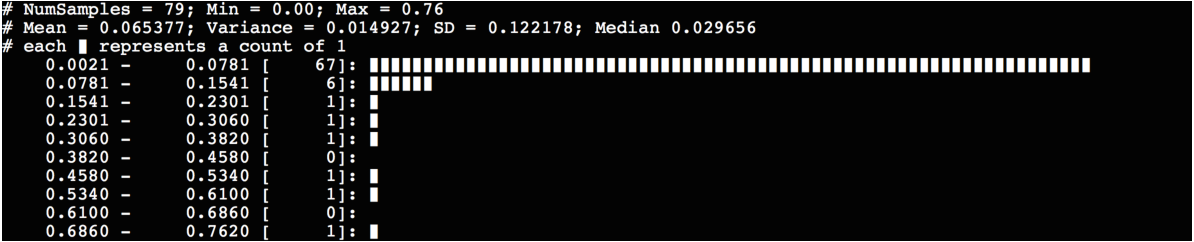
\includegraphics[width=0.90\textwidth]{evgen1.pdf}
 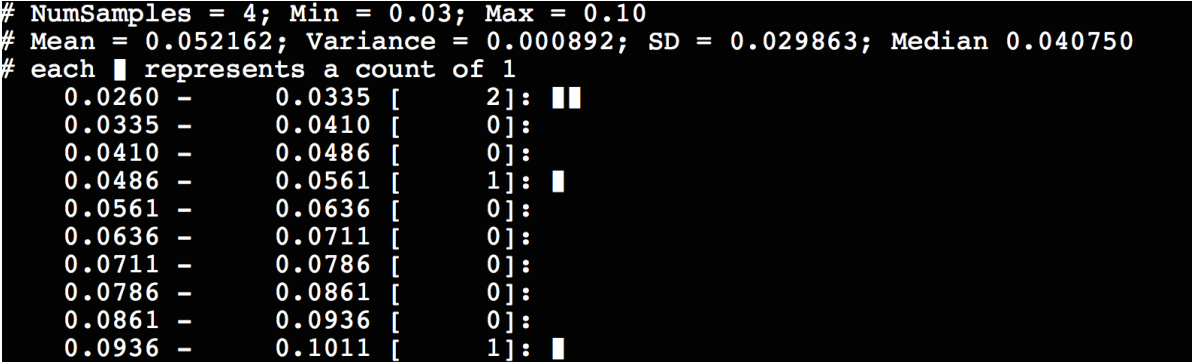
\includegraphics[width=0.60\textwidth]{evgen2.pdf}
 \caption{\small The number of MC events from the $4j$ background sample at the end of
   the cut-based analysis, in the resolved (upper plot) and boosted (category), distributed
   according to their associated MVA output.
}
\label{fig:evgen}
\end{center}
\end{figure}
%%%%%%%%%%%%%%%%%%%%%%%


   However, it is always important to validate expectations in a explicit way, so we have increased
   by a factor 10 the size of our $2b2j$ and $4j$ Monte Carlo background samples, up to a total
   of 30M each.
   %
   These have been used to repeat the analysis with a more reliable estimate of the $2b2j$ and $4j$
   background cross-sections, specially  relevant for the later.
   %
   In this case, the number of $4j$ signal events
   that pass the cuts (level C2, before MVA) is around 1000 in the resolved category
   and around 100 in the boosted,
   which provides a  more robust estimate of the multijet background cross-section.

   We would like to emphasize here that repeating the full analysis with the high-statistics background samples would be already very
   CPU-time intensive, and a further increase of the background stats is beyond our
   computing power. For instance, generating  300M events of the $2b2j$ and $4j$ samples would take around a couple months running on 50 cores. And for at analysis level, already with O(100M) background events the analysis
   time with PU included
   would take around one month running on 25 cores full time, becoming clearly unfeasibly
   if the number of background events is further increased to  O(1000M).


 \item The final remark from the referee is the following:

   \begin{quote}
     \it ``Along the same line, the authors give fake-rates for the different backgrounds in Table 5 and conclude at the end of section 4.2 that the multi-jet backgrounds can be neglected. However, with a fake rate of
     $10^{-4}$ \%, the $4j$ background would still correspond to 1 pb I do not see how this can be neglected when studying a signal of few fb.''
   \end{quote}

   We agree that this statement is not as precise as it could be.
   %
   What we meant here was the following: consider for instance Table 4, in the resolved category,
   before the application of $b$-tagging.
   %
   At this level of the cut flow,
   the cross-sections in fb for the QCD multijet background are
   $1.6\cdot 10^4$, $3.2\cdot 10^6$ and $2.1\cdot 10^7$ fb for $4b$, $2b2j$ and $4j$
   respectively.
   %
   Now, after the application of naive fake $b$-tagging probabilities, these numbers
   should be multiplied by $1,10^{-4},10^{-8}$ respectively, which would make
   the $2b2j$ and $4j$ cross-sections
   much smaller than $4b$.

  
   However the actual probabilities are those of Table 5 of the
   original manuscript: applying these
   we find cross-sections after $b$-tagging of around 1.2 pb, 1.3 pb and 50 fb respectively.
   %
   This means that in the resolved category, chosen here for illustration, the $4j$ background
   is smaller than the $2b2j$ and $4b$ backgrounds by at least an order of magnitude (consistent
   with the row C2 of the resolved category of C2) and thus is unlikely to play a major
   role in the estimation of the overall signal significance.
  
\end{itemize}


To validate the robustness of our original results, 
we have redone the complete analysis with the updated background samples
in the case without PU, including
the MVA (re-)training.
%
This way, it is possible to compare the signal significances found
in this updated analysis with those that are reported in the original manuscript.

  First of all, in Table~\ref{tab:cutflow_noPU_1} of this reply
  we show the comparison of the signal and total background
      cross-sections at the end of the cut-based analysis (level C2),
      between the original and the updated analysis,  for the resolved (upper),
      intermediate (middle) and boosted
      (lower table) categories, in the case of the analysis
      without PU.
      %
      As can be seen, there is good agreement between the original and the updated
      estimates of the background cross-sections at the end of the cut-based analysis,
      with the updated values being somewhat larger due to both the additional single-Higgs
      backgrounds included and the improved modelling of the QCD multijet component.

  %%%%%%%%%%%%%%%%%%%%%%%%%%%%%%%%%%%%%%%%%%%%%%%%%
\begin{table}[h!]
  \centering \small
   \begin{tabular}{|l|cc|}
  \hline
\multicolumn{3}{|c|}{HL-LHC, Resolved category, no PU}\\
\hline
&  \multicolumn{2}{c|}{Cross-section [fb]}  \\
   &  $hh4b$ &  total bkg \\
  \hline
  C2, original analysis    & 0.5  &   $4.9\cdot 10^3$        \\
  C2, updated analysis    & 0.5  &   $7.0\cdot 10^3$        \\
\hline
   \end{tabular}\\
   \vspace{0.5cm}
    \begin{tabular}{|l|cc|}
  \hline
\multicolumn{3}{|c|}{HL-LHC, Intermediate category, no PU}\\
\hline
&  \multicolumn{2}{c|}{Cross-section [fb]}  \\
   &  $hh4b$ &  total bkg \\
  \hline
  C2, original analysis    &  0.09  &  $1.8\cdot 10^2$        \\
  C2, updated analysis    &  0.09  &  $2.8\cdot 10^2$      \\
\hline
    \end{tabular}\\
     \vspace{0.5cm}
    \begin{tabular}{|l|cc|}
  \hline
\multicolumn{3}{|c|}{HL-LHC, Boosted category, no PU}\\
\hline
&  \multicolumn{2}{c|}{Cross-section [fb]}  \\
   &  $hh4b$ &  total bkg \\
  \hline
  C2, original analysis    &   0.16  &   $2.5\cdot 10^2$       \\
  C2, updated analysis    &    0.16  &   $3.1\cdot 10^2$       \\
\hline
   \end{tabular}
%%%%%%%%%%%%%%%%%%%%%%%%%%%%%%%%%%%%%%%%%%%%%%%%%%%%%%%%%%%%%%%
    \caption{\small Comparison of the signal and total background
      cross-sections at the end of the cut-based analysis (level C2),
      between the original and the updated analysis,  for the resolved (upper),
      intermediate (middle) and boosted
      (lower table) categories, in the case of the analysis
      without PU.
      %
 \label{tab:cutflow_noPU_1}}
\end{table}


  %%%%%%%%%%%%%%%%%%%%%%%%%%%%%%%%%%%%%%%%%%%%%%%%%%%%%%%%%%%%%%%%%%%%%%%%%%%%
\begin{table}[h]
  \centering
  \begin{tabular}{|c|l|c|c|c|c|c|}
    \hline
    \multicolumn{7}{|c|}{HL-LHC, no PU} \\
    \hline
    \hline
    Category  &  Analysis & ANN cut & $N_{\rm ev}$ signal &  $N_{\rm ev}$ back  &  $S/\sqrt{B}$ & $S/B$ \\ 
    \hline
    \hline
    \multirow{2}{*}{Boosted} & Original & $y_{\rm cut}=0.90$ &  290  & $1.2\cdot 10^4$   & 2.7  & 0.03 \\
    & Updated & $y_{\rm cut}=0.80$ & 140    &   $1.9\cdot 10^3$   &  3.2   &  0.07  \\
    \hline
    \hline
    \multirow{2}{*}{Intermediate} &   Original & $y_{\rm cut}=0.85$ & 130  & 3100  & 2.3 & 0.04\\
     &   Updated & $y_{\rm cut}=0.75$ & 30  &  260  & 1.7   & 0.11 \\
    \hline
    \hline
    \multirow{2}{*}{Resolved} & Original  & $y_{\rm cut}=0.60$ & 630 & $1.1\cdot 10^{5}$  & 1.9 & 0.01 \\
        & Updated & $y_{\rm cut}=0.50$ & 230  & $2.7\cdot 10^{5}$   & 1.4  & 0.01  \\
    \hline
      \end{tabular}
  \caption{\small
Same as Table 6 of the original paper, containing the post-MVA
results for the optimal value of the
ANN discriminant, where we now compare the numbers from the original
analysis with those of the updated analysis described in this reply.
    %
    We quote the number of signal and
    background events expected for $\mathcal{L}=3$ ab$^{-1}$,
    the signal significance $S/\sqrt{B}$ and
    the signal over background ratio $S/B$.
    %
    We also quote the value of the ANN cut $y_{\rm cut}$ used in this case, though their
    values are not quite comparable since the distribution of the events in the ANN output
    is different in the updated analysis as compared to the original analysis (different MVA training).
    %
    \label{tab:mva}
  }
\end{table}
%%%%%%%%%%%%%%%%%%%%%%%%%%%%%%%%%%%%%%%%%%%%%%%%%%%%%%%%%%%%%%%%%%%%%%%%%%%%

%
Next, in Table~\ref{tab:mva} we provide the same
information as Table 6 of the original paper, containing the post-MVA
results for the optimal value of the
ANN discriminant, where we now compare the numbers from the original
analysis with those of the updated analysis described in this note.
    %
    We quote the number of signal and
    background events expected for $\mathcal{L}=3$ ab$^{-1}$,
    the signal significance $S/\sqrt{B}$ and
    the signal over background ratio $S/B$.
    %
    Note that due to the MVA re-training on the updated background samples
    (both the high-stats QCD multijets and the single-higgs background) the determination
    of the optimal value of the cut on the ANN discriminant on each category needs
    to be performed again independently.
    %
    In particular, we find that now tighter cuts (leading to a reduced number
    of signal events passing the MVA cut) are
    required to achieve similar signal significance, most likely
    due to the more robust population of the phase space from the
    QCD multijet backgrounds.
    %
    This reduces the overall number of signal events to be observed
    at the HL-LHC down to around 400, though we also now find larger values
    of $S/B$ in the boosted and resolved categories,
    which is also an important requirement.

    As we can read from Table~\ref{tab:mva}, we achieve a similar signal significance combining the three
    categories:
    \be
   \lp \frac{S}{\sqrt{B}}\rp_{\rm tot} = 4.0 \quad {\rm original~analysis}
   \ee
    \be
   \lp \frac{S}{\sqrt{B}}\rp_{\rm tot} = 3.9 \quad {\rm updated~analysis}
   \ee
   implying that the conclusions derived
   in the original analysis are essentially unchanged following the improved treatment
   of the background processes.

   All the cross-checks listed in this note
   make us confident that the signal significances claimed in our
   manuscript are robust enough, and therefore there is no need to update all the tables
   and plots in our analysis (which in the case of PU is beyond our computing resources),
   due to the fact that the overall physics message would be unchanged.
%
  In any case, we are already working on a follow-up paper about the determination of the Higgs trilinear coupling, and there all the modifications that are reported here will be documented in detail.

\end{document}

%%%%%%%%%%%%%%%%%%%%%%%%%%%%%%%%%%%%%%%%%%%%%%%%%%%
%%%%%%%%%%%%%%%%%%%%%%%%%%%%%%%%%%%%%%%%%%%%%%%%%%%
